\begin{figure*}[!htb]
\minipage{0.31\textwidth}
  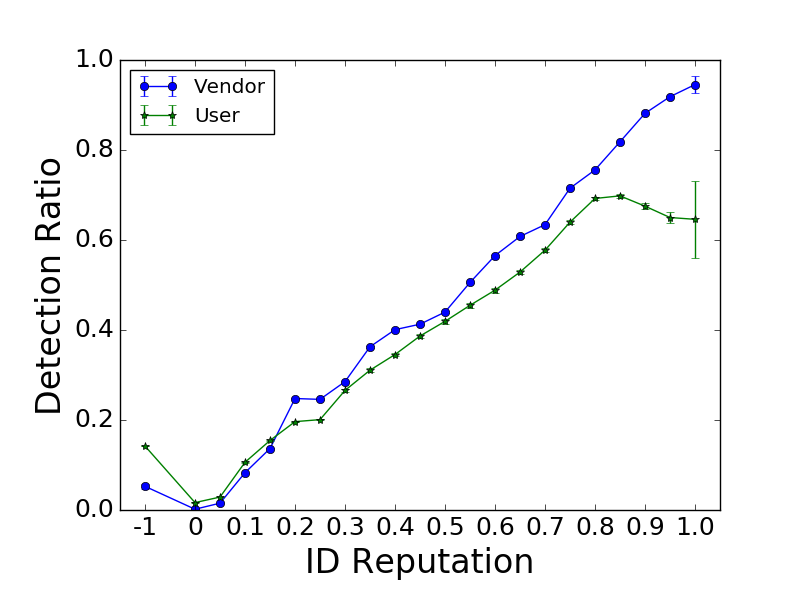
\includegraphics[width=\linewidth]{figure/IDReputation}
  \mycaption{fig:idreputation}{The relation between source id's previous reputation and detection rate.}
{\footnotesize{(How detection rate changes with the value of source id's reputation. Each reputation is rounded up to nearest 0.05.
Reputation -1 means the source id did not make any submission before. 95\% confidence interval is also drawn 
for each point.)}}
\endminipage\hfill
\minipage{0.31\textwidth}
  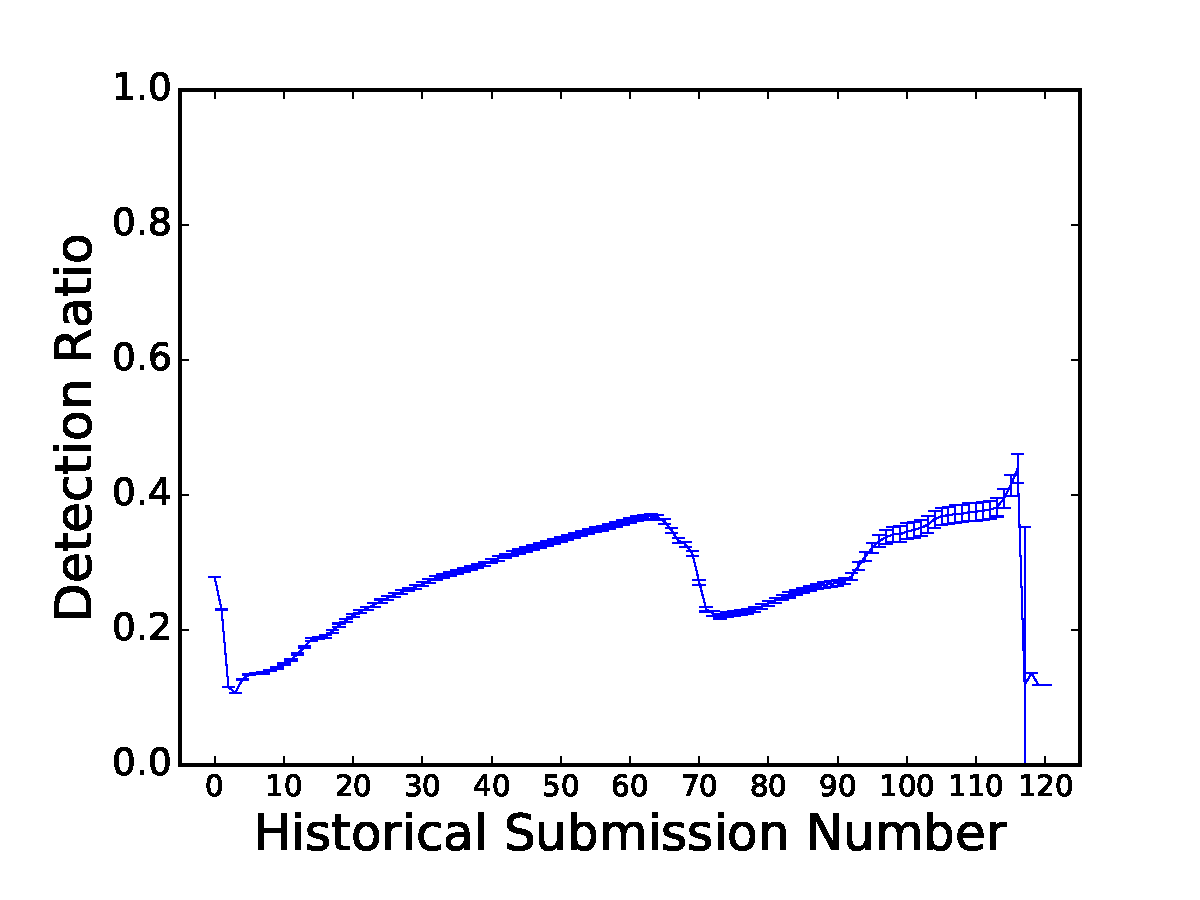
\includegraphics[width=\linewidth]{figure/SubNum}
  \mycaption{fig:hisnum}{The relation between historical submission number and detection rate.}
  {\footnotesize{(How detection rate changes with historical submission number. 
Each historical number is rounded up to nearest 5.
95\% confidence interval is also drawn for each point.)}}
\endminipage\hfill
\minipage{0.31\textwidth}%
  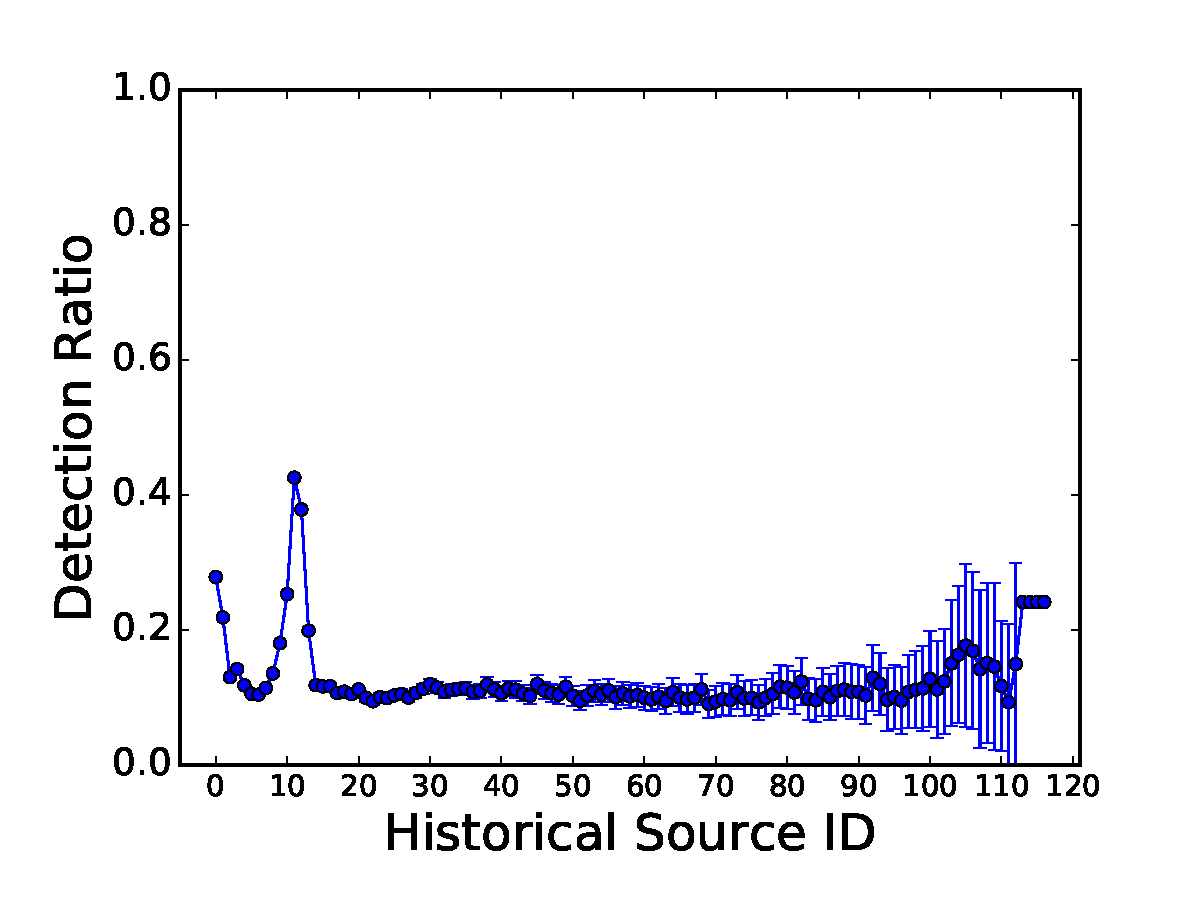
\includegraphics[width=\linewidth]{figure/SubID}
  \mycaption{fig:hisid}{The relation between the number of historical source ids and detection rate.}
{\footnotesize{(How detection rate changes with the number of historical source ids. 
Each historical number of source ids is rounded up to nearest 5.
95\% confidence interval is also drawn for each point.)}}
\endminipage\hfill

%\vspace{-0.2in}
\end{figure*}

\begin{figure*}[!htb]
\minipage{0.31\textwidth}
  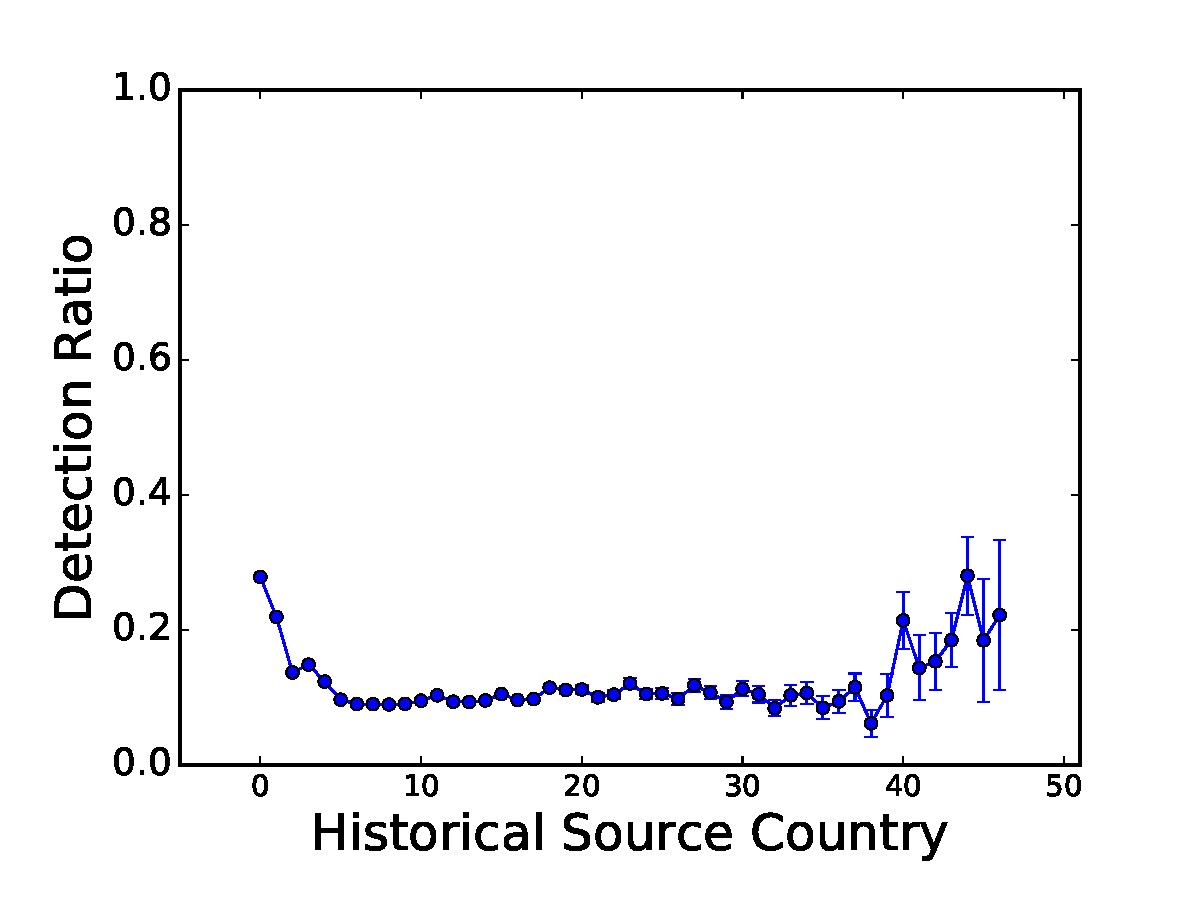
\includegraphics[width=\linewidth]{figure/SubCountry}
  \mycaption{fig:hiscountry}{The relation between the number of historical source countries and detection rate.}
{\footnotesize{(How detection rate changes with the number of historical source countries.
95\% confidence interval is also drawn for each point.)}}
\endminipage\hfill
\minipage{0.31\textwidth}
  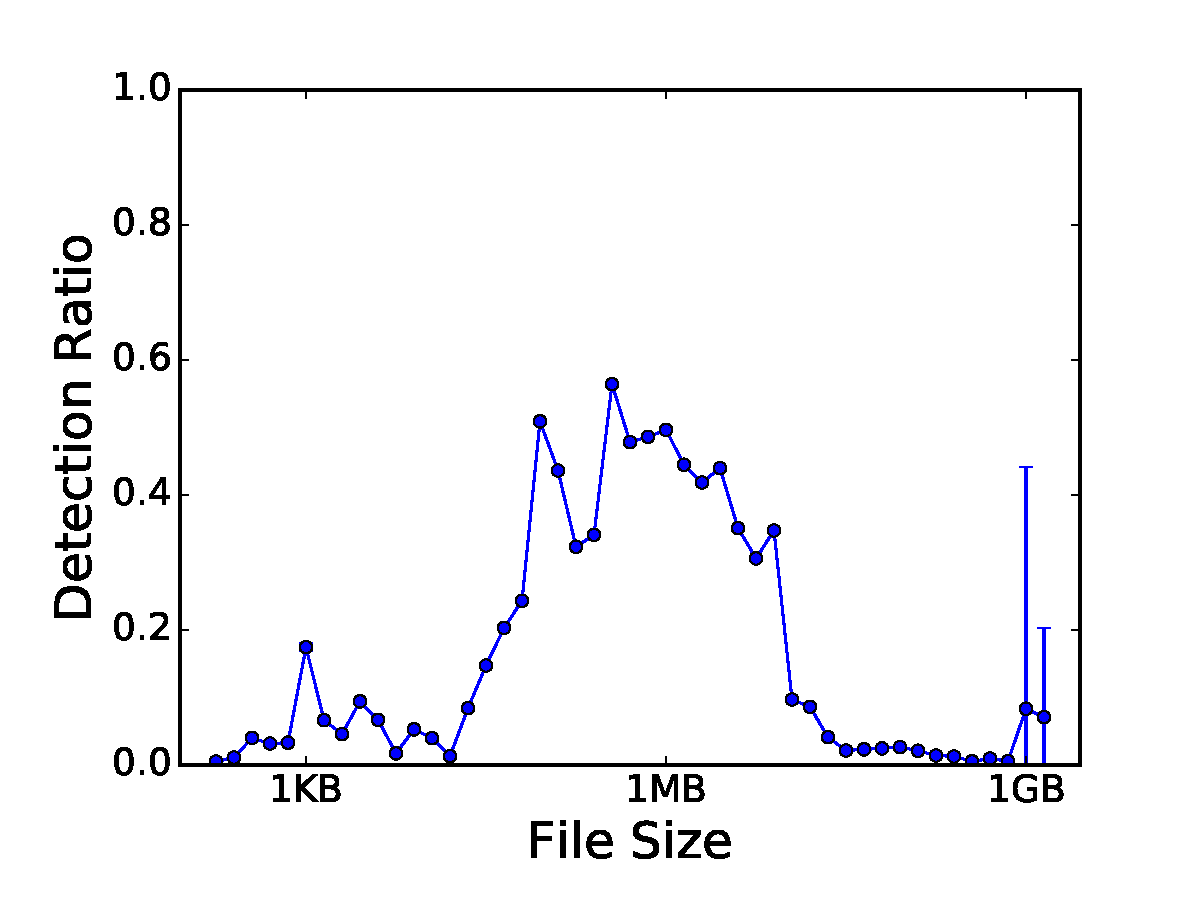
\includegraphics[width=\linewidth]{figure/size}
  \mycaption{fig:size}{How detection rate changes with file size.}
  {\footnotesize{(How detection rate changes with log2-based file size.
Results from log2 are rounded up to nearest 0.5.
95\% confidence interval is also drawn for each point.)}}
\endminipage\hfill
\minipage{0.31\textwidth}%
  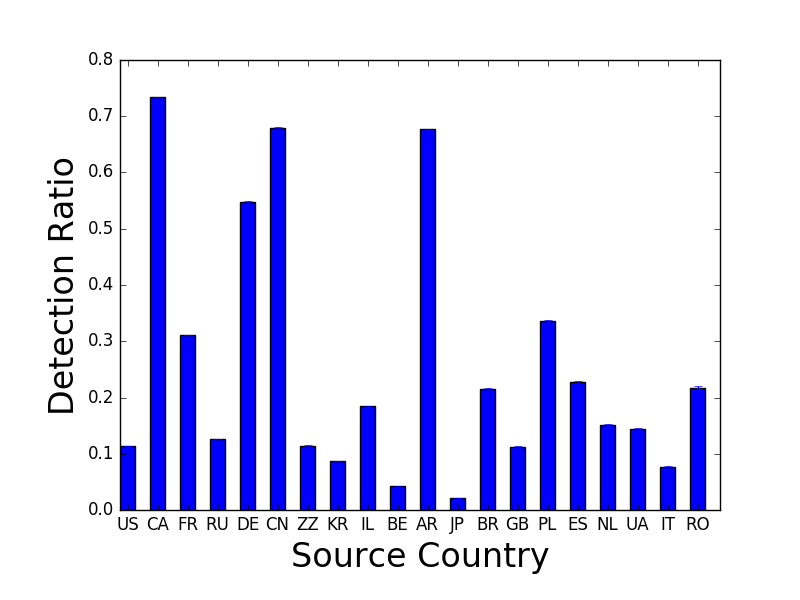
\includegraphics[width=\linewidth]{figure/Country}
  \mycaption{fig:Country}{Average detection rate for top 20 countries.}
{\footnotesize{(Average detection rate for submissions from countries ranking 
in top 20 in making PE submissions to VirusTotal. 
95\% confidence interval is also drawn for each country.)}}
  %\label{fig:aveUncover}
\endminipage\hfill

%\vspace{-0.2in}
\end{figure*}